\section{Empirical study of the joint dynamics of the implied volatility and its underlying index}\label{sec:empirical_study}

\subsection{Data sets}\label{sec:data}
We consider two data sets of daily implied volatility surfaces sourced from two different data providers. The first one corresponds to options on the S\&P 500 index while the second one corresponds to options on the Euro Stoxx 50. Both data sets start on March 8, 2012 and end on December 30, 2022. They contain the at-the-money-forward (denoted by ATM in the sequel for the sake of simplicity) implied volatilities for time-to-maturities ranging from 1 month to 24 months with a monthly timestep. For the same range of time-to-maturities, the S\&P 500 data set also contains the implied volatilities for values of forward moneyness ranging from 0.6 to 1.4 with a 0.01 step while the Euro Stoxx 50 contains the implied volatilities for Black-Scholes deltas in the following range: \textpm 0.1, \textpm 0.15, \textpm 0.2, \textpm 0.25, \textpm 0.3, \textpm 0.35, \textpm 0.4, \textpm 0.45 (positive deltas correspond to calls while negative deltas correspond to puts). As a remainder, the Black-Scholes delta corresponds to the sensitivity of the option price with respect to the price of the underlying asset. Its formula  (assuming zero dividend) is recalled below:
\begin{equation}\label{eq:delta_formula}
    \Delta^{BS} = \epsilon\mathcal{N}(\epsilon d_1) \text{ with } d_1 = \frac{\ln\frac{S_0}{K}+(f_T+\frac{\sigma^2}{2})T}{\sigma \sqrt{T}}
\end{equation}
where $\mathcal{N}$ is the cumulative normal distribution function, $\epsilon=1$ for call options and $-1$ for put options, $K$ is the strike, $T$ the time-to-maturity, {$f_T$ is the continuously compounded forward rate for the time-to-maturity $T$} and $\sigma$ the Black-Scholes implied volatility. In the sequel of this section, we only focus on the ATM implied volatilities but, in Sections \ref{sec:svi} and \ref{sec:pdv_ssvi}, the away-from-the-money implied volatilities will also be used. Let us emphasize that these two data sets do not consist of raw data of market calls and puts prices but result from a pre-processing which is at the discretion of the data providers. Indeed, options with the above time-to-maturities are not traded every day on the market. For example, on the Chicago Board Options Exchange where calls and puts on the S\&P 500 are traded, the following options are traded at day $t$:
\begin{enumerate}
    \item \textbf{Weekly expiry options:} options expiring every business day between $t$ and $t+28$ business days. Note that before 2022, there was only Monday-, Wednesday- and Friday-expiring options. 
    \item \textbf{End-of-Month options:} options expiring the last business day of the month for up to twelve months after $t$. 
    \item \textbf{Monthly expiry options:} options expiring the third Friday of the month for a given range of future months up to 5 years after $t$. 
\end{enumerate}
A similar decomposition can be found for options written on the Euro Stoxx 50 on the Eurex but with differences in the expiry dates (for example, there are only Weekly expiry options that expire on Fridays). \\

Along with these two IVSs data sets, we also have daily time series of the S\&P 500 and Euro Stoxx 50 indices. The S\&P 500 time series starts on January 2, 1980 while the Euro Stoxx 50 time series starts on December 31, 1986 and both end on December 30, 2022. Note that since we will use at most 12 years of past returns to predict the implied volatility, the whole time series are not used in the following study.  \\

To measure the out-of-sample performance of the tested model, we split the two data sets into a train set and a test set: the train set spans the period from March 8, 2012 to December 31, 2020 and the test set spans the period from January 1, 2021 to December 30, 2022 so that approximately 80\% of the data is used for the train and 20\% is used for the test. In addition, we will also consider a blocked cross-validation in Section \ref{sec:influence_cutoff}. The 1-month ATM implied volatility along with the underlying asset price are represented in Figure \ref{fig:data_sets} for both data sets. 

\begin{figure}[t]
    \centering
    \subfigure[S\&P 500]{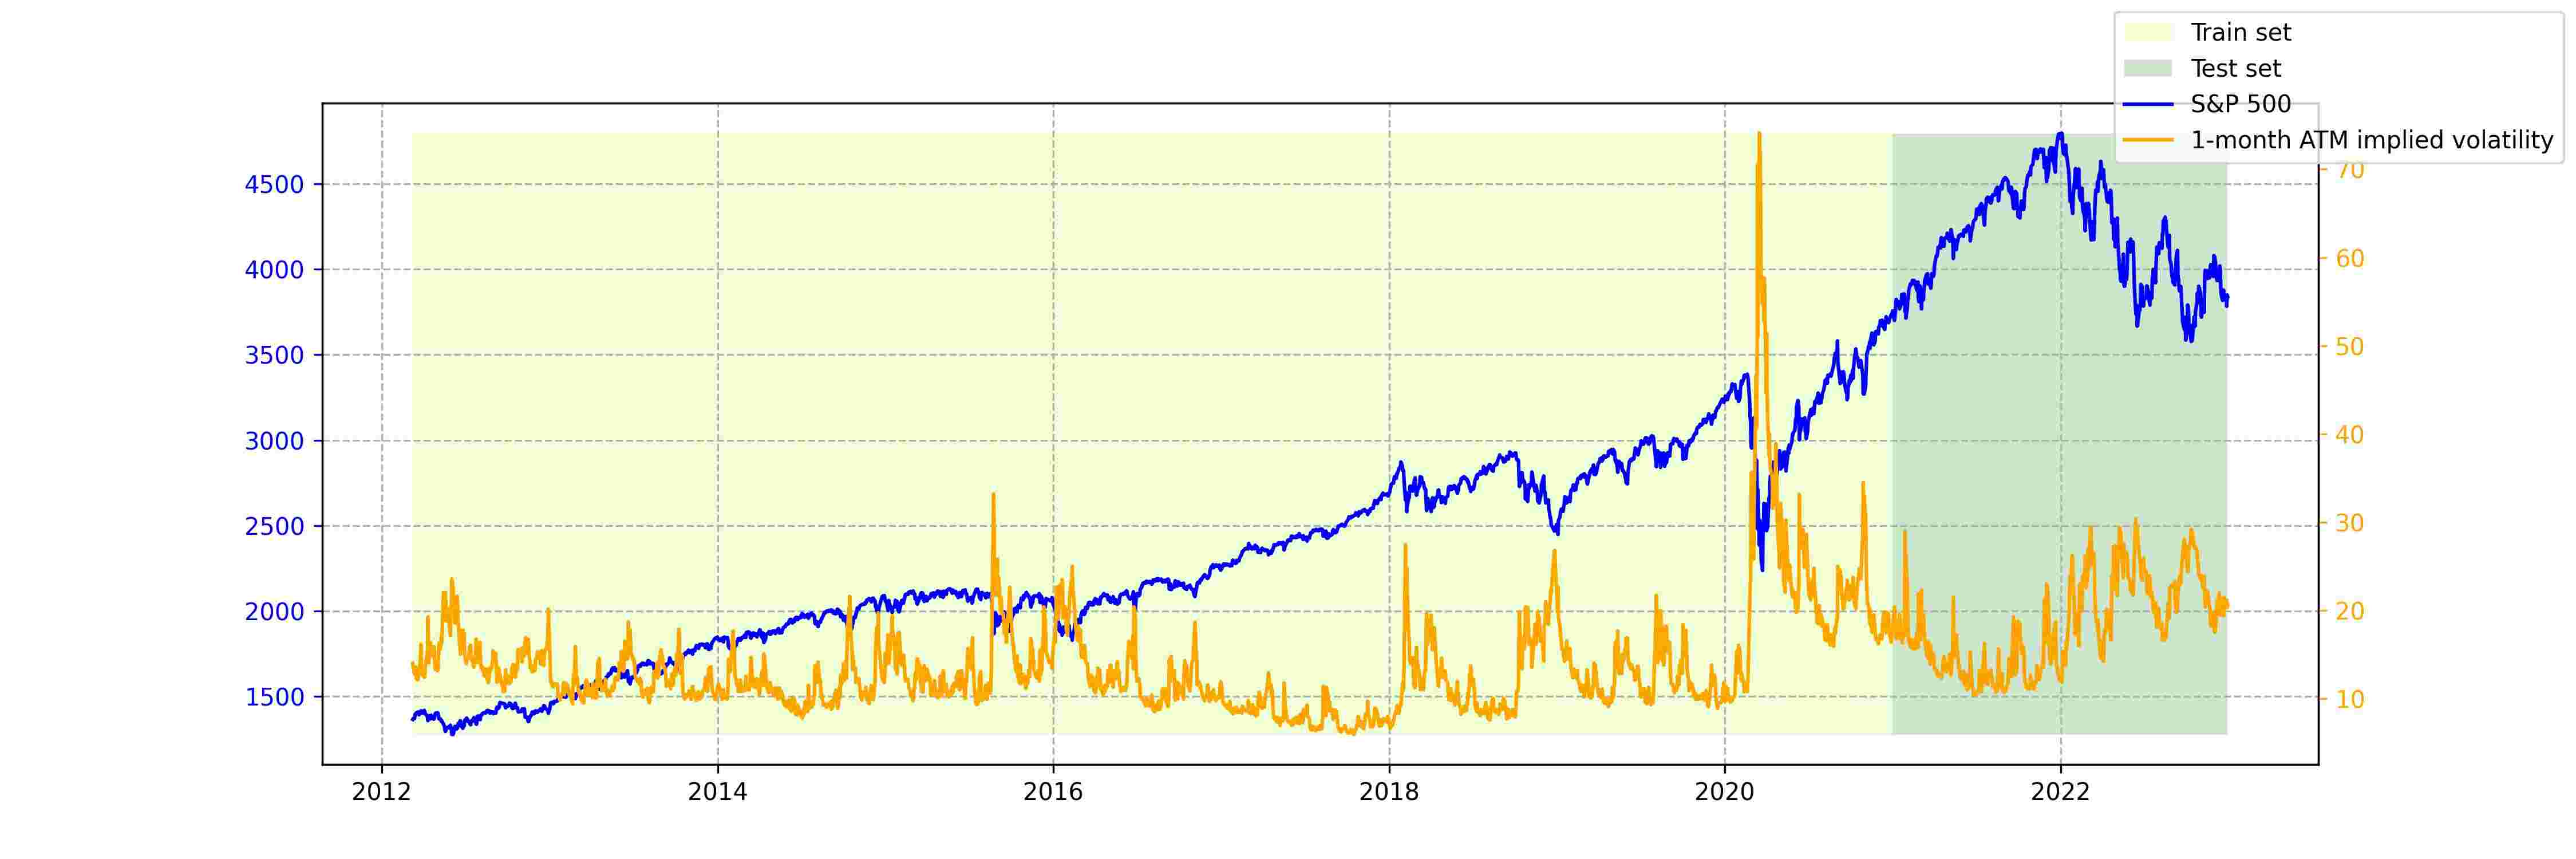
\includegraphics[width=\linewidth]{SPX_IV.jpg}}
    \subfigure[Euro Stoxx 50]{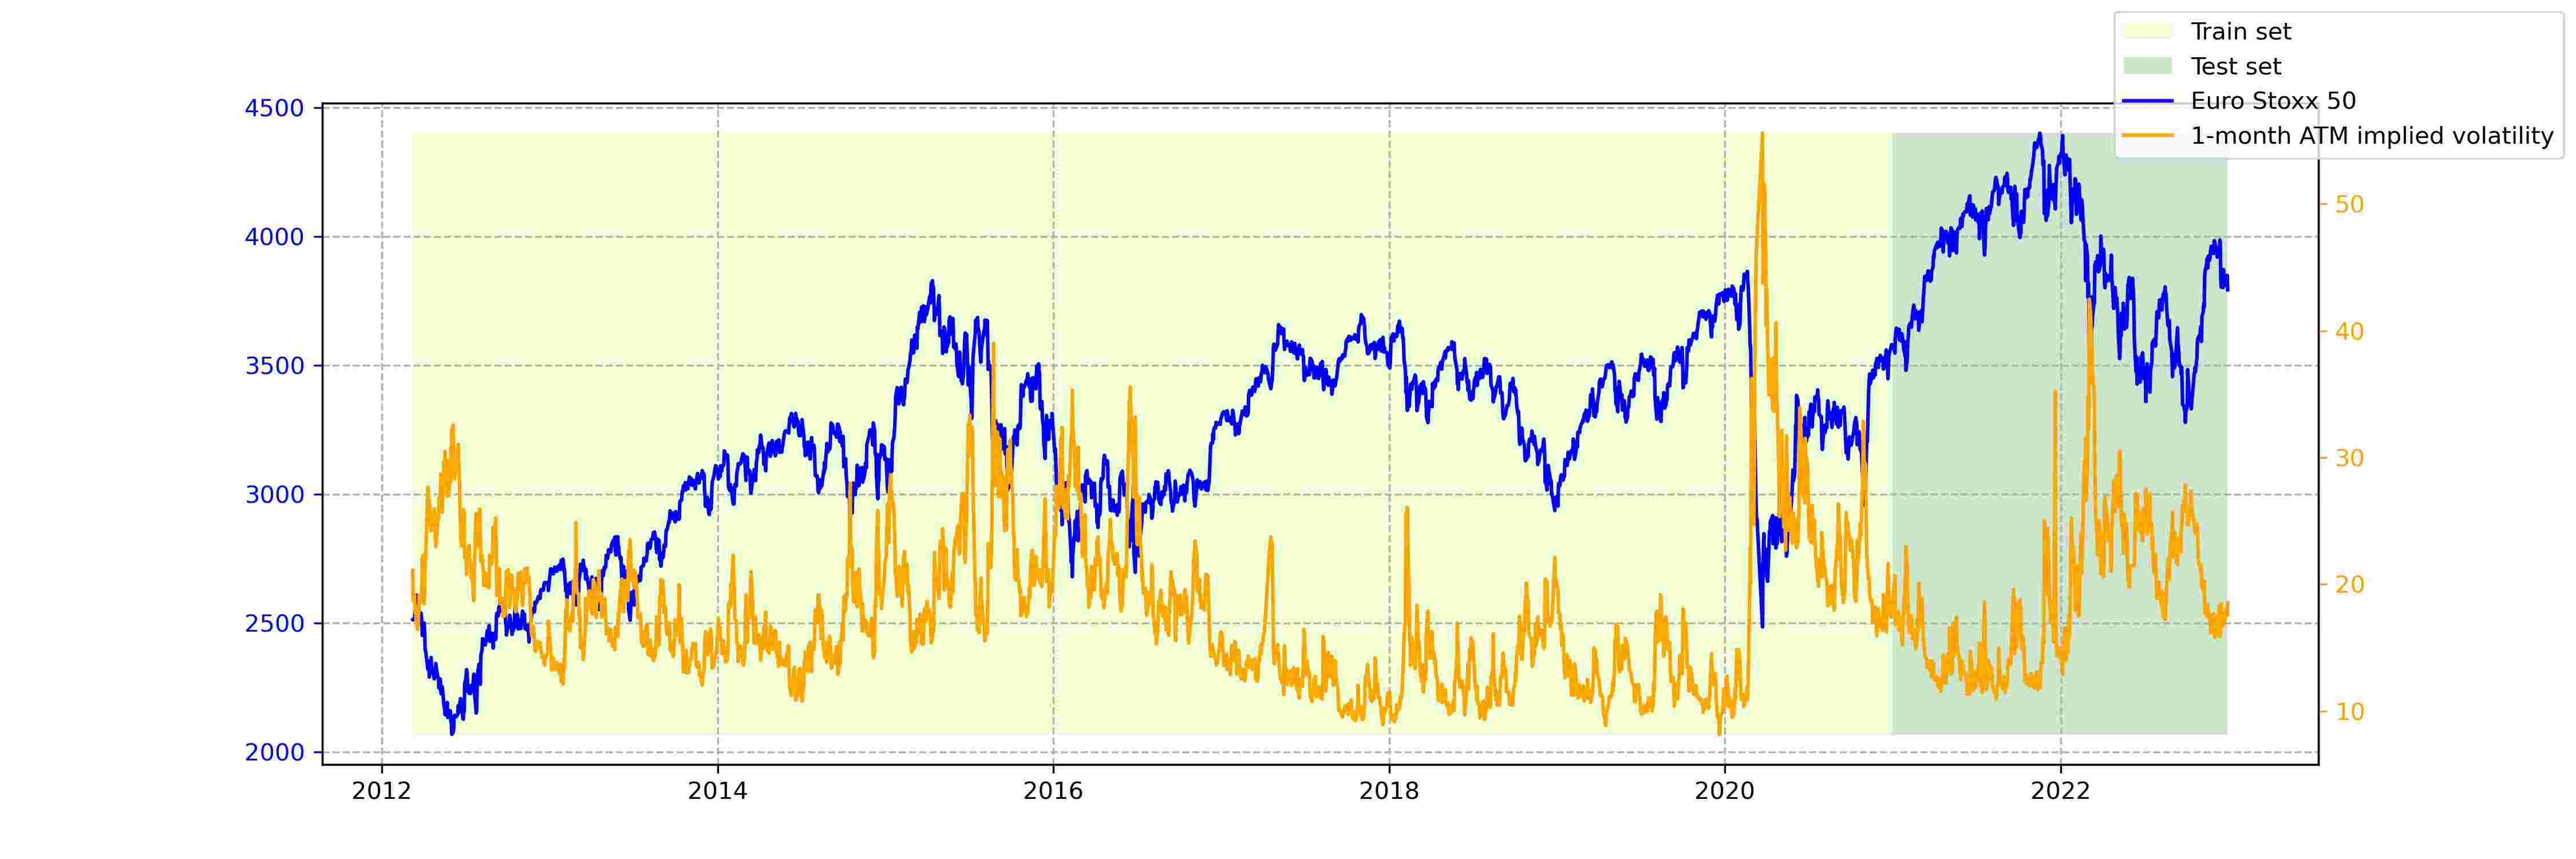
\includegraphics[width=\linewidth]{SX5E_IV.jpg}}
    \caption{Joint evolution of the 1-month ATM implied volatility and its underlying index from March 8, 2012 to December 30, 2022. The split between the train and the test sets is represented through the use of different background colors.}
\label{fig:data_sets}
\end{figure}

\subsection{Calibration methodology} \label{sec:calib_meth}
The PDV model (\ref{eq:guyon_model}) with the TSPL kernel relies on 7 parameters, namely $(\alpha_1,\delta_1,\alpha_2,\delta_2)$ the parameters of the two TSPL kernels $K_1$ and $K_2$ (Equation (\ref{eq:tspl_kernel})) and $(\beta_0,\beta_1,\beta_2)$, respectively the intercept, the sensitivity to the trend feature and the sensitivity to the volatility feature. These 7 parameters are calibrated specifically for each time-to-maturity using the following steps (which are identical to the ones implemented by \cite{guyon2022volatility} to which we refer for more details\footnote{See also the code provided with their paper: \url{https://github.com/Jordylek/VolatilityIsMostlyPathDependent}}):
\begin{enumerate}
    \item We compute four exponentially weighted moving averages (EWMA) with respective spans of 10, 20, 120 and 250 days of the underlying index returns. Then, we run a ridge regression of the ATM implied volatility on the four EWMAs and we fit the TSPL kernel $K_1$ on the optimal linear combination of the exponential kernels which provides us with initial guesses for $\alpha_1$, $\delta_1$. The use of a ridge regression instead of a lasso regression is justified by the fact that we do not need to maximize the number of zeros (i.e. minimize the number of exponential kernels) in view of the subsequent fit of a TSPL kernel. By running a ridge regression of the ATM implied variance on four EWMAs of the underlying index squared returns and fitting the TSPL kernel $K_2$, we obtain similarly initial guesses for $\alpha_2$ and $\delta_2$.  
    \item Initial guesses for $\beta_0$, $\beta_1$ and $\beta_2$ are then obtained using a linear regression of the ATM implied volatility on the features $R_1$ and $\Sigma$ where $\alpha_1$, $\delta_1$, $\alpha_2$ and $\delta_2$ are fixed to the values estimated at step 1. 
    \item Starting from these initial guesses, the 7 parameters are jointly calibrated by solving the following minimization problem using the \texttt{least\_squares} function with the trust-region reflective algorithm from the \texttt{scipy} Python package:
    \begin{equation}\label{eq:target_fun}
        \begin{array}{rrrlll}
        \displaystyle\min_{(\alpha_1,\delta_1,\alpha_2,\delta_2,\beta_0,\beta_1,\beta_2) \in \mathbb{R}^7} & \multicolumn{5}{c}{\displaystyle\sum_{t\in \mathcal{T}_{train}} (IV^{mkt}_t - \beta_0-\beta_1R_{1,t}-\beta_2\Sigma_t)^2 } \\
       \text{s.t.} & \alpha_j, \delta_j &\ge& 0 \text{ for } j \in \{1,2\} \\
       &R_{1,t} &=& \displaystyle\sum_{t-C\le t_i \le t} \frac{Z_{\alpha_1,\delta_1}}{(t-t_i+\delta_1)^{\alpha_1}} r_{t_i} \\
      &\Sigma_{t} &=& \sqrt{\displaystyle\sum_{t-C\le t_i \le t} \frac{Z_{\alpha_2,\delta_2}}{(t-t_i+\delta_2)^{\alpha_2}} r_{t_i}^2}
        \end{array}
    \end{equation}
    where $\mathcal{T}_{train}$ is the set of dates in the train set, $IV^{mkt}_t$ is the market ATM implied volatility observed at time $t$ for some fixed time-to-maturity and $C$ is a cut-off lag. 
\end{enumerate}

\subsection{Numerical results}\label{sec:empirical_study_numerical_results}
% They calibrate this model both on implied volatility indices and realized volatilities and obtain $R^2$ scores above 85\% both on train and test sets for the implied volatility and $R^2$ scores above 50\% for the realized volatilities. The remainder of this section is an empirical study of the model on implied volatilities instead of volatility indices.
\subsubsection{Performance of the PDV model}\label{sec:overall_perf}
We start by calibrating the PDV model (\ref{eq:guyon_model}) using the methodology described in Section \ref{sec:calib_meth}. Note that the computation of the features $R_1$ and $\Sigma$ requires to truncate the sums at some point parameterized by $C$. While we use for the moment the previous 1,000 business days (i.e. $C=1000$), consistently with the choice of \cite{guyon2022volatility}, the influence of this hyperparameter will be discussed in Appendix \ref{sec:influence_cutoff}. The performance of the model is measured using the $R^2$ score (the definition is recalled in Equation (\ref{eq:r2})) which allows to assess how much of the variance of the implied volatility is explained by the model. The results are presented in Figure \ref{fig:r2_cutoff_1000}. For the S\&P 500, we obtain $R^2$ scores between 86\% and 95\% on the train set, between 68\% and 83\% for the 15 first time-to-maturities and between 55\% and 68\% for the last time-to-maturities on the test set. For the Euro Stoxx 50, we obtain $R^2$ scores between 85\% and 90\% on the train set, between 70\% and 81\% for the 15 first time-to-maturities and between 50\% and 70\% for the last time-to-maturities on the test set. These results indicate that a large part of the movements of the ATM implied volatility can be explained by the past movements of the underlying asset price. In this regard, they extend those of \cite{guyon2022volatility} to ATM implied volatility data. We also notice that the $R^2$ scores are overall decreasing with the option time-to-maturity: this is quite natural as we expect long-term options to be less sensitive to the variations of the underlying asset price than short-term options. This observation is also consistent with the results of \cite{bakshi2000call} who noticed that 'the longer an option’s remaining life, the more likely its price goes in the opposite direction with the underlying asset' suggesting that there is more exogeneity in the evolution of the prices of long-term options than in those of short-term options. \\

\begin{figure}[h]
    \centering
    \subfigure[S\&P 500]{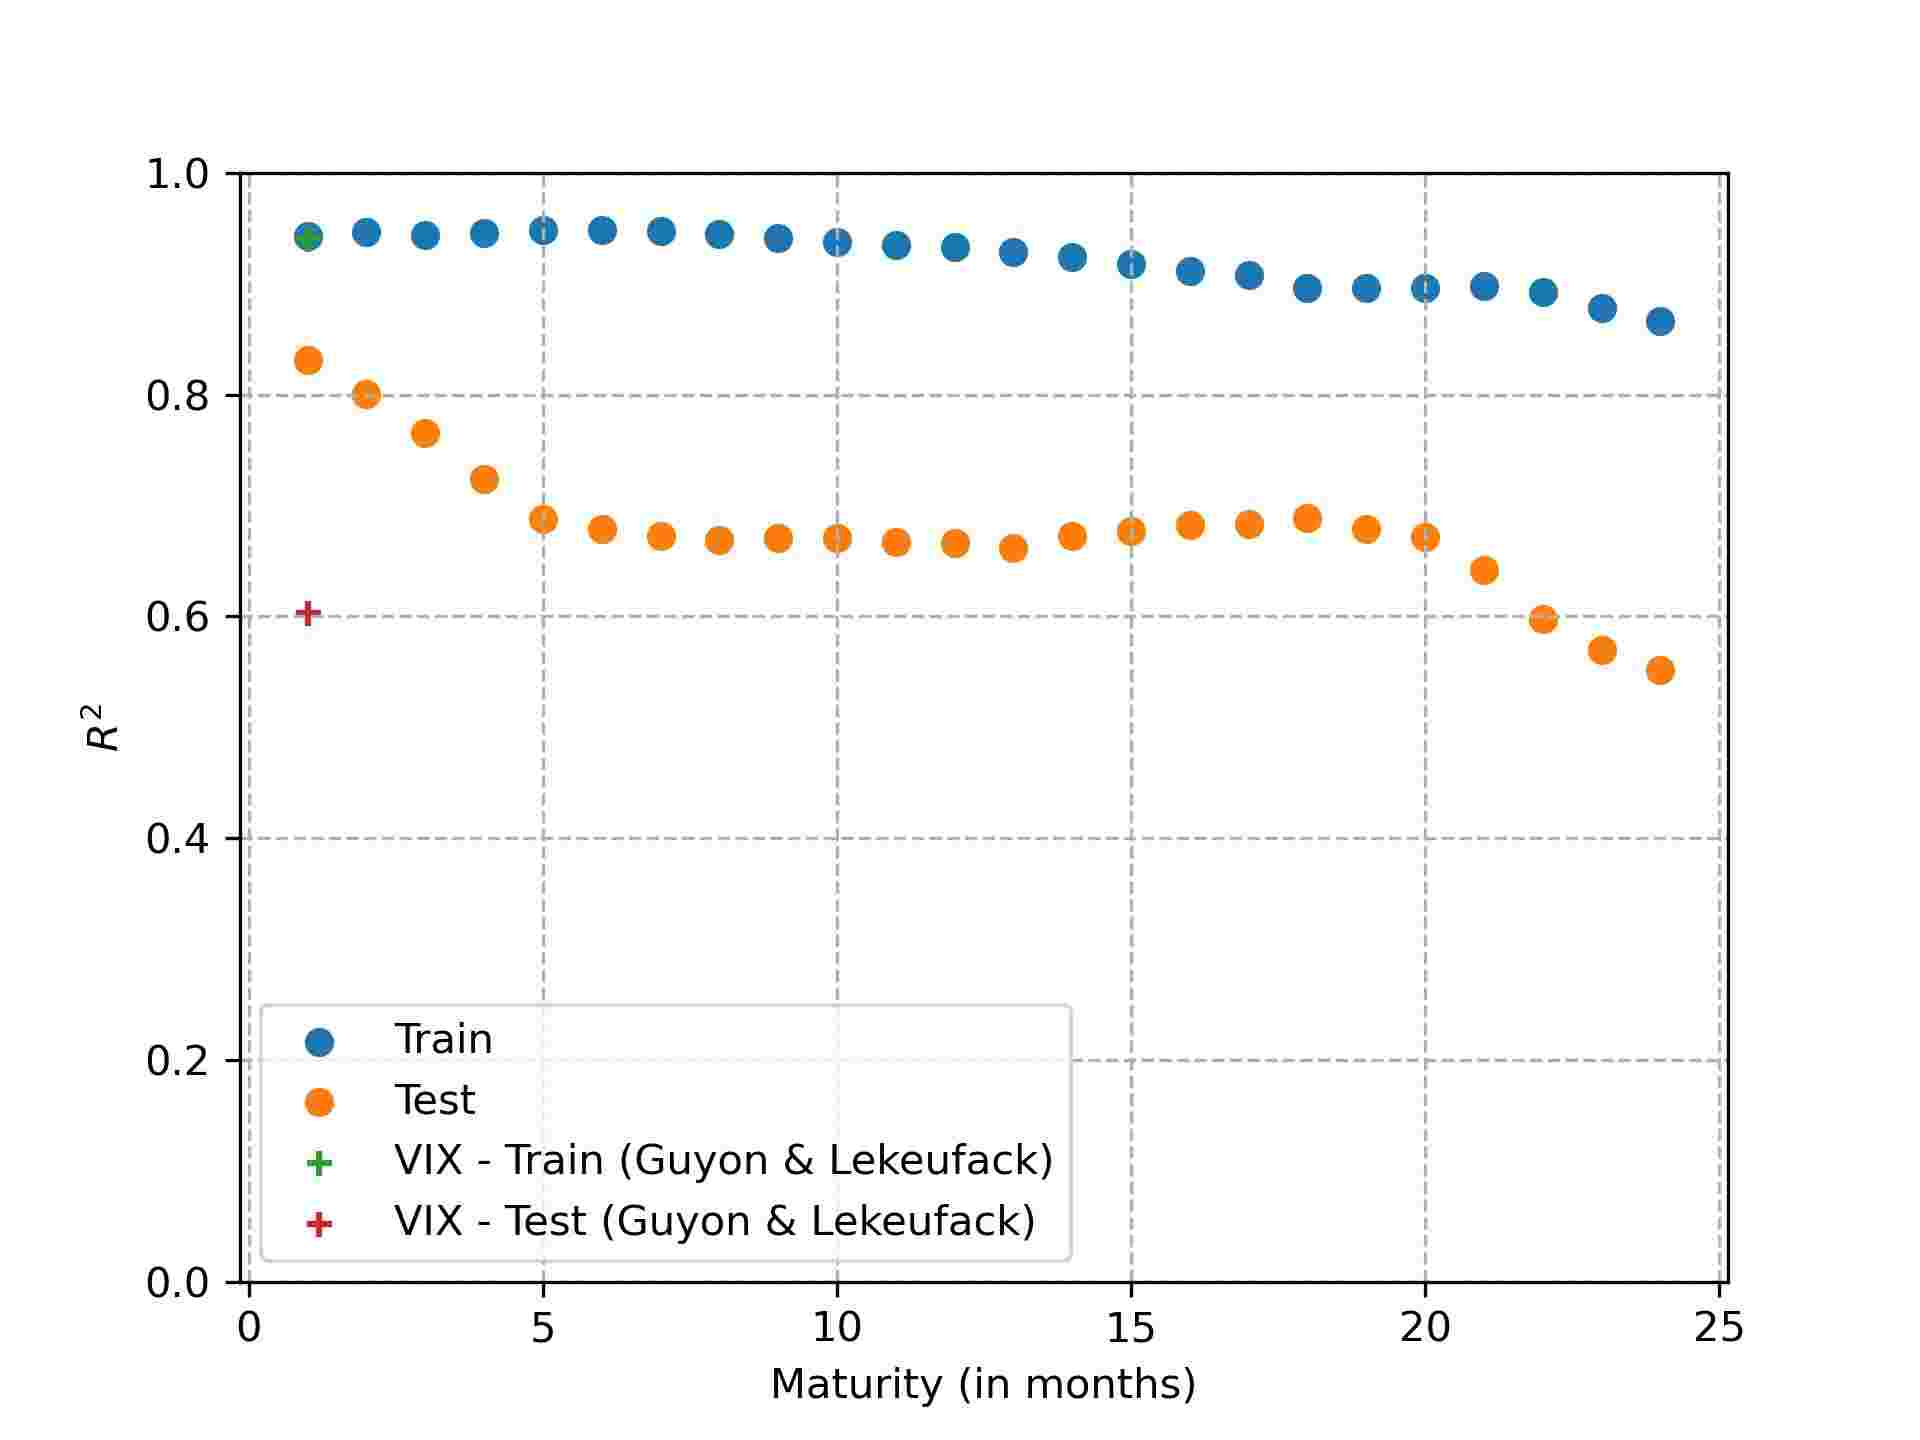
\includegraphics[width=0.45\linewidth]{SPX_Scores_Cutoff_1000.jpg}}
    \subfigure[Euro Stoxx 50]{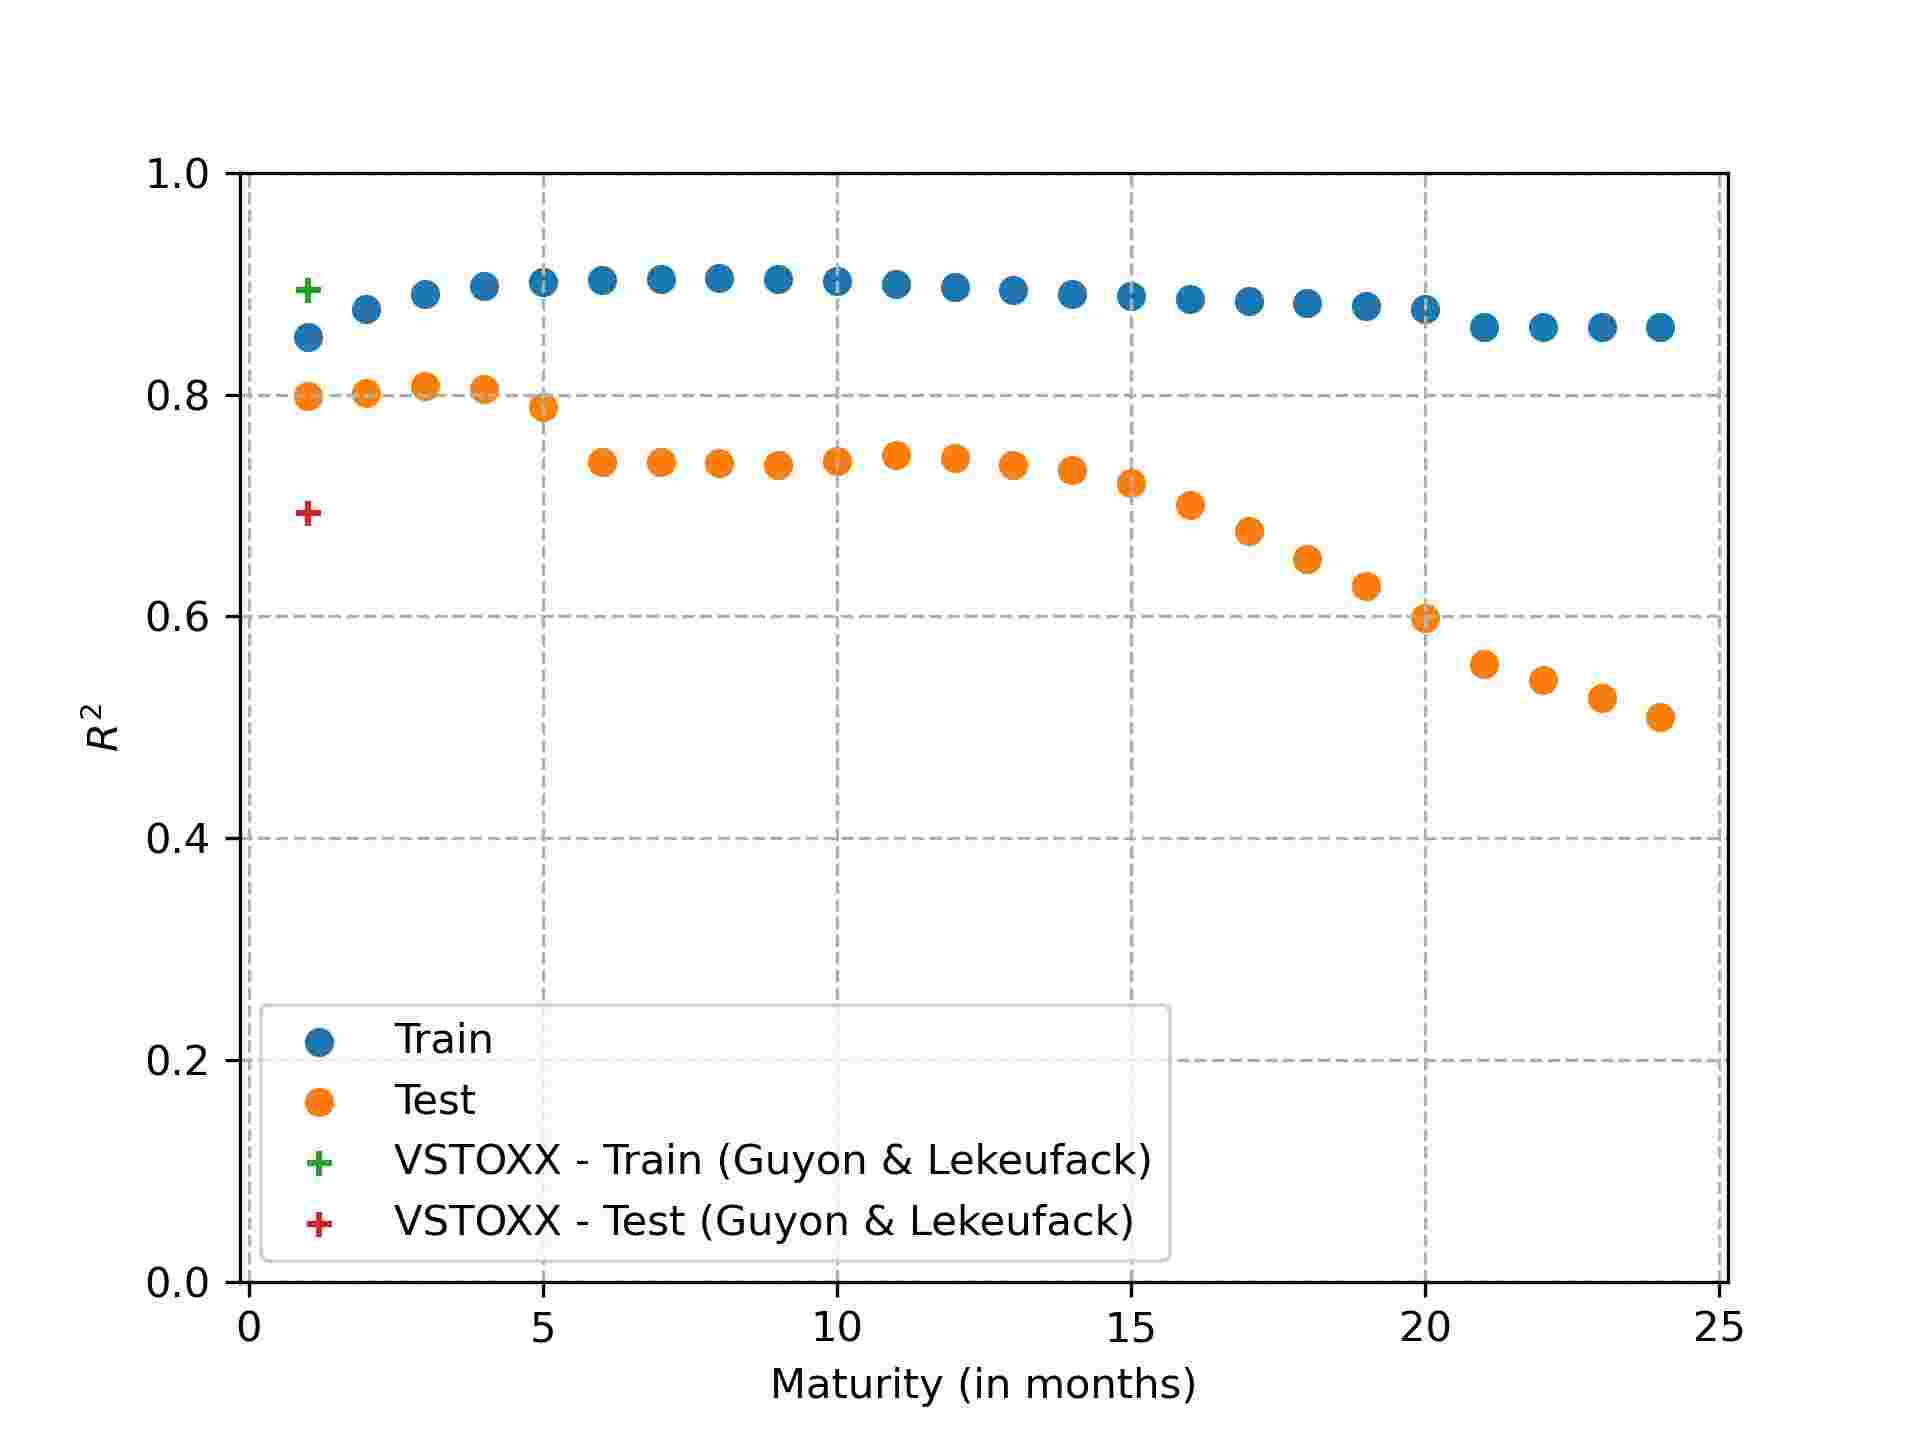
\includegraphics[width=0.45\linewidth]{STXE_Scores_Cutoff_1000.jpg}}
    \caption{$R^2$ scores on the train and the test sets as a function of the ATM implied volatility time-to-maturity. The average $R^2$ scores for the VIX and the VSTOXX are also displayed.}
\label{fig:r2_cutoff_1000}
\end{figure}
The two following subsections deepen the analysis of Figure \ref{fig:r2_cutoff_1000}. 

\subsubsection{Comment on the gap between the scores on the train and the test sets}\label{sec:comment_gap}
We observe a gap of approximately 24\% for the S\&P 500 and 19\% for the Euro Stoxx 50 between the $R^2$ scores on the train set and the test set. Such gaps are usually symptomatic of overfitted models. However, if we keep only one feature to reduce the complexity of the model, be it the trend feature $R_1$ or the volatility feature $\Sigma$, the $R^2$ scores are lower (especially with the trend feature) and the gap between the train and the test sets widens. Another way to deal with overfitting is to add a regularization term in the objective function. Such a technique is implemented in Appendix \ref{sec:influence_cutoff} but does not reduce the gap between the performance on the train and the test sets. Because of these two arguments, we estimate that the observed gap is not the result of an overfitted model but rather the result of the fact that the test set is both small (only 2 years of data) and of a peculiar nature. Indeed, the test set corresponds to the post-Covid-19 period which is characterized by a lot of uncertainty related to the Russia-Ukraine war, inflation, the rise of interest rates, etc. which may have affected the extent to which the volatility reacts to the underlying index movements. For the S\&P 500, the difference between the evolution on the train set and the test set is very clear: apart from the crash of March 2020, the S\&P 500 has experienced a constant increase with very little variations on the train set while the test set is characterized by a bull market followed by a bear market with high volatility. Note that the difference between the periods is however less clear for the Euro Stoxx 50. To support the claim that the test set is of peculiar nature, we compute the ratio $D$ of the signed distances and the absolute distances between the observed implied volatilities and the predicted implied volatilities on the test set:
\begin{equation}
    D = \frac{\displaystyle\sum_{t\in \mathcal{T}_{test}} IV_t^{mkt} -\beta_0-\beta_1R_{1,t}-\beta_2\Sigma_t }{\displaystyle\sum_{t\in \mathcal{T}_{test}} \left| IV_t^{mkt} -\beta_0-\beta_1R_{1,t}-\beta_2\Sigma_t \right|}
\end{equation}
where $\mathcal{T}_{test}$ is the set of dates in the test set. This indicator allows to measure whether there are more implied volatility observations above ($D>0$) or below ($D<0$) the plane fitted on the train set. Considering the 1-month implied volatilities, we obtain a ratio of 13.7\% for the S\&P 500 and 4.1\% for the Euro Stoxx 50. This suggests that most data points lie above the plane, implying a stronger reaction of the implied volatility to the movements in the underlying index during the post-Covid 19 period. Another possible reason of the gap between the scores on the train and the test sets is the high autocorrelation of the residuals of the PDV model which are given by $IV_t^{mkt-\beta_0-\beta_1R_{1,t}-\beta_2\Sigma_t}$. Indeed, the autocorrelation of the residuals at lag 1 day lies at 89\% (average over the autocorrelations of the residuals for the 24 time-to-maturities) and it is still above 26\% at lag 50 days, indicating a long memory. This high positive autocorrelation of the residuals implies that the predicted implied volatility is sometimes always above the observed implied volatility and sometimes always below. This can lead to low $R^2$ scores if the time period considered for the calculation of these $R^2$ scores is not large enough as it is the case here.

% \begin{figure}[h]
%     \centering
%     \subfigure[Calibration using only the trend feature. ]{\includegraphics[width=0.45\linewidth]{SPX_Scores_Trend_Feature.jpg}}
%     \subfigure[Calibration using only the volatility feature.]{         \includegraphics[width=0.45\linewidth]{SPX_Scores_Volatility_Feature.jpg}}
%     \caption{$R^2$ scores on the train and the test sets of the S\&P 500 as a function of the ATM implied volatility time-to-maturity for the PDV model with only one feature.}
% \label{fig:r2_one_feature}
% \end{figure}

% \begin{figure}[h!]
%     \centering
%     \subfigure[S\&P 500]{\includegraphics[width=0.45\linewidth]{SPX_test_prediction.jpg}}
%     \subfigure[Euro Stoxx 50]{\includegraphics[width=0.45\linewidth]{SX5E_test_prediction.jpg}}
% \caption{1-month ATM implied volatility level on the test set as a function of the trend feature $R_1$ and the volatility feature $\Sigma$. The plane corresponds to the predicted values when the PDV model is fitted on the train set and the green dots correspond to the data points.}
% \label{fig:test_prediction}
% \end{figure}

\subsubsection{Comparison with the scores of \cite{guyon2022volatility}}
In Figure \ref{fig:r2_cutoff_1000}, we also represent (with green and red crosses) the $R^2$ scores obtained when calibrating the PDV model on the VIX and the VSTOXX (which are the volatility indices of the S\&P 500 and the Euro Stoxx 50 respectively) using the same historical time period (from March 8, 2012 to December 30, 2022). They allow a consistent comparison between our scores and those of \cite{guyon2022volatility}. Note that the scores are represented at the same abscissa as the scores obtained on the 1-month implied volatilities. This choice is motivated by the fact that both the VIX and the VSTOXX are measures of the 30-days expected variance of their respective underlying index. We observe that the $R^2$ scores on the test set for the volatility indices are: 
\begin{enumerate}
    \item below the scores for the 1-month implied volatility and 
    \item below the scores reported by \cite{guyon2022volatility} for the same indices (the difference being only the train and test periods: their train and test sets respectively span the periods from January 1, 2000 to December 31, 2018 and from January 1, 2019 to May 15, 2022 while our train and test sets respectively span the periods from March 8, 2012 to December 31, 2020 and from January 1, 2021 to December 30, 2022).
\end{enumerate}
The first observation shows that the 1-month ATM implied volatility is even better predicted by the PDV than the volatility indices considered by \cite{guyon2022volatility}. The second observation confirms that the $R^2$ scores of the PDV model are quite sensitive to the choice of the train and test sets as discussed in Section \ref{sec:comment_gap}. \\

The empirical study conducted in this section allowed us to exhibit the dependence of the ATM implied volatility on the past path of the underlying asset price for two major financial indices. We showed that this dependence decreases with the time-to-maturity but remains material even for the largest time-to-maturities. At this stage, it is natural to ask whether these conclusions still hold for away-from-the-money implied volatilities. Instead of reproducing the empirical study for each time-to-maturity and strike (which would increase significantly the dimension of the study), we study the performance of the PDV model in explaining the evolution of the calibrated parameters of the SSVI parameterization of \cite{gatheral2014arbitrage}. The following section is dedicated to the presentation of this parameterization. 

